The impedance of whole cells can also be used to calculate important parameters of microorganisms. The single-shell and two-shell models generally used for the simulation of biological cells in an aqueous solution can be approximated as simple charged particles in suspension in a solution considering their relative magnitude compared to the bulk fluid \cite{Xu2016}. The simplest model for a biological cell with a lipid layer plasma membrane is the “single-cell” model \cite{asami2002characterization,Gawad2004,morgan2006single,Sun2010,Xu2016} modelled by a homogeneous phase cytoplasm and an insulating thin shell, as shown in \autoref{fig:CellModel}. Bacteria, yeast, and plant cells are examples of microorganisms that possess a cell wall outside of the plasma membrane. This addition modifies the single shell model to a double shell model. A similar kind of analysis as the single-shelled model can be done, which is described in detail in \citep{asami2002characterization} \cite{Xu2016}. Maxwell’s mixture theory can be applied to obtain the equivalent complex permittivity of the mixture following these equations \cite{Xu2016,morgan2006single}:
\begin{equation}
   \varepsilon_{mix} = \frac{\varepsilon_m (1+2\phi f_{CM})}{1-\phi f_{CM}}
\end{equation}

\begin{equation}
   f_{CM} = \frac{\varepsilon_c - \varepsilon_m}{\varepsilon_c + 2\varepsilon_m}
\end{equation}

\begin{equation}
   \phi = \frac{4}{3} \pi R^3 \frac{1}{\kappa w l h}
\end{equation}
\begin{figure}[h]
    \centering
    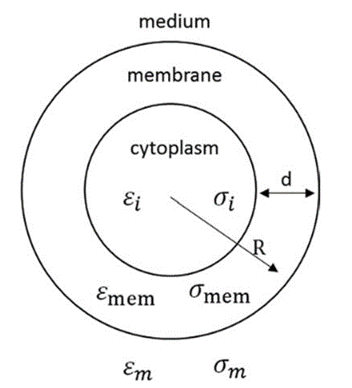
\includegraphics[width=0.4\textwidth]{CellModel}
    \caption{Electrical model of a single-shelled cell suspended in a medium. \citep{simscale_2021}}
    \label{fig:CellModel}
\end{figure}
Where $\varepsilon_m$ , $\varepsilon_c$, and $\varepsilon_{mix}$ are respectively the complex permittivity of the medium, cell, and cell-medium mixture. $\phi$ represents, the volume fraction of the cell to the detection area, $f_{CM}$ the Clausis-Mossotti factor, $h$ the height of the channel, $R$ the cell radius, $\kappa$ the cell constant, and $w$ and $l$ are the width and length of the coplanar electrodes, respectively. This equation can be used to determine the single-shelled spherical cell model, which describe the cell permittivity \cite{Xu2016,morgan2006single} $\varepsilon_c$ as :
\begin{equation}
\epsilon_c = \frac{\varepsilon_{memb} (\rho ^3 + 2 \frac{\varepsilon_i-\varepsilon_m}{\varepsilon_i+2\varepsilon_m})}{\rho ^3- \frac{\varepsilon_i-\varepsilon_m}{\varepsilon_i+2\varepsilon_m}}
\end{equation}

Where $\varepsilon_{memb}$ and $\varepsilon_{i}$ represent the permittivity of the cell membrane and cell cytoplasm, and $\rho$ describe a ratio between the membrane thickness $d$ and cell radius $R$. \par

The permittivity of the medium, membrane, and cytoplasm are fundamental properties of cells, meaning that they can be used to catalog between different species. The complex permittivity is a function that depends on frequency. The choice of the excitation signal’s frequency depends on the properties targeted by the analysis. \citep{Schwan1963} distinguished between three ranges of frequency for biological cells in suspension in a liquid, named $\alpha$, $\beta$, and $\gamma$ dispersions. Frequencies below several kilohertz constitute those in the $\alpha$-dispersion and are mostly affected by electrode polarization effects caused by the EDL \cite{grahame1947electrical}, as well as ionic diffusion. The $\gamma$-dispersion is found at frequencies above 1 GHz and behaves accordingly to the reorientation of water molecules (which are dipolar) present in the SUT \cite{Hasted1973}. The $\beta$-dispersion lies in between the frequency from the $\alpha$ and $\gamma$ regions and features a fair amount of useful information for the whole cell measurements and interfacial polarization \cite{Caselli2010}. Indeed, the impact of the EDL, the cell’s size, the cell’s membrane, and the cell’s cytoplasm are all observable in this zone, as shown in \autoref{fig:CellFrequency}. This makes the $\beta$-dispersion the zone which is generally used for impedance-based cell measurements \cite{Xu2016,Opitz2019}.
\begin{figure}[h]
    \centering
    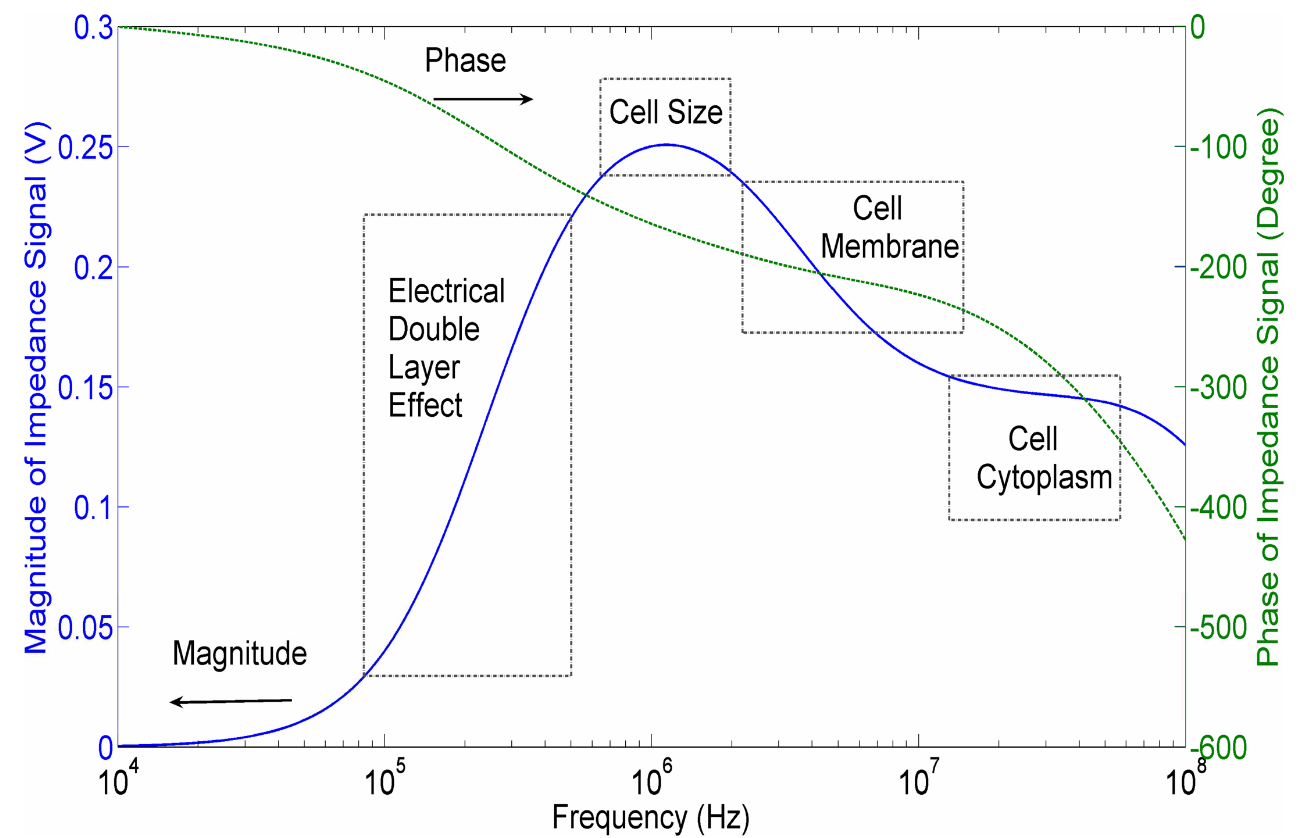
\includegraphics[width=0.9\textwidth]{CellFrequency}
    \caption{Impedance magnitude and phase variations of a single-shelled cell obtained from PSpice simulations. \citep{sun2008analytical}}
    \label{fig:CellFrequency}
\end{figure}